\chapter{Background and Related Works}
The purpose of code generation tools is to help developers improve their productivity, ensure correctness of code syntax, and lessen the number of errors in software \cite{groher_01}.  The input specifications of these tools introduce additional levels of indirection to solve these problems \cite{spinellis_01}.  A range of tools have been created to generate code that can be complex and tedious to write by hand:
\begin{itemize}
  \item Scanners
  \item Parsers
  \item Interpreters
  \item Compilers
  \item Graphical user interfaces
\end{itemize}

\section{Scanner and Parser Code Generation}
The Yacc compiler-compiler \cite{johnson_01} first introduced in 1975 generates LALR parsers that must be run with a lexical analyzer generator such as Lex.  Similar to Yacc is Bison \cite{aycock_01,demaille_01}—a Yacc-compatible parser generator that accepts any properly written Yacc grammar.  Like Yacc, Bison-generated parsers read a sequence of tokens from a scanner generated by a lexical analyzer generator like Lex or flex.

\indent
To illustrate the steps of traditional parser generation using Lex and Yacc (figure ~\ref{fig:YaccGrammarRule}) \cite{johnson_01,lesk_01,niemann_01}, a file is provided by the developer containing a set of patterns that define how to separate strings found in source data.  This file is read by Lex, which uses these patterns to generate the C source code of a lexical analyzer.  This newly generated lexical analyzer uses the patterns to identify specific strings in the input and split them into tokens to simplify processing.

\begin{figure}[htbp]
\centering
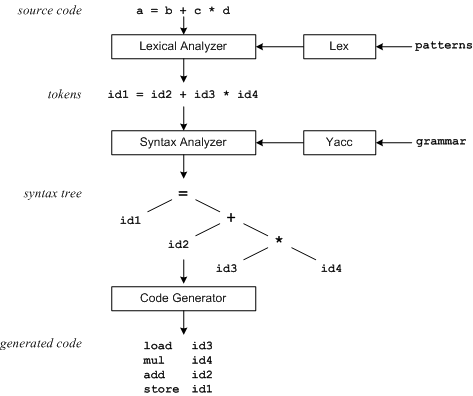
\includegraphics[width=0.9\textwidth]{figures/LexAndYaccCompileSequence.png}
\caption[Lex and Yacc Compilation Sequence]{Lex and Yacc Compilation Sequence \cite{niemann_01}}
\label{fig:LexAndYaccCompileSequence}
\end{figure}

\indent
A file containing grammar rules is provided by the developer to Yacc, which uses those rules to generate C source code for a syntax analyzer (i.e. parser).  The syntax analyzer uses this grammar to transform the tokens output by the lexical analyzer into a syntax tree.  The structure of this syntax tree implies the precedence and associativity of operators found within the tokens.  The syntax tree is then traversed in depth-first order to generate the desired source code (figure ~\ref{fig:LexAndYaccCompileSequence}) \cite{niemann_01}.

\indent
A predicated-LL(k) parser called ANTLR \cite{parr_01} was introduced by Parr and Quong in 1995.  The ANTLR parser generator was advertised to be easier to use than generators like YACC or BISON.  An LL(k) parser is a top-down parser that parses from left to right, utilizing a look-ahead of k tokens.  All parsing decisions are made solely from the next k tokens, which means that it does no backtracking.

\indent
The HYACC (Hawaii Yacc) parser generator first released in 2008 supports complete LR(0), LALR(1), LR(1), and partial LR(k) \cite{chen_01,chen_02}.  HYACC is compatible with Yacc and Bison input grammars and works with Lex.  The HYACC parser generator is notable because it can resolve reduce/reduce conflicts through its implementation of the LR(1) parser generation algorithm \cite{chen_01}.  Reduce/reduce conflicts occur when two or more rules in an input grammar apply to the same input sequence \cite{free_01}.  These conflicts are typically the result of a serious problem with an input grammar \cite{free_01}.

\begin{figure}[htbp]
\centering
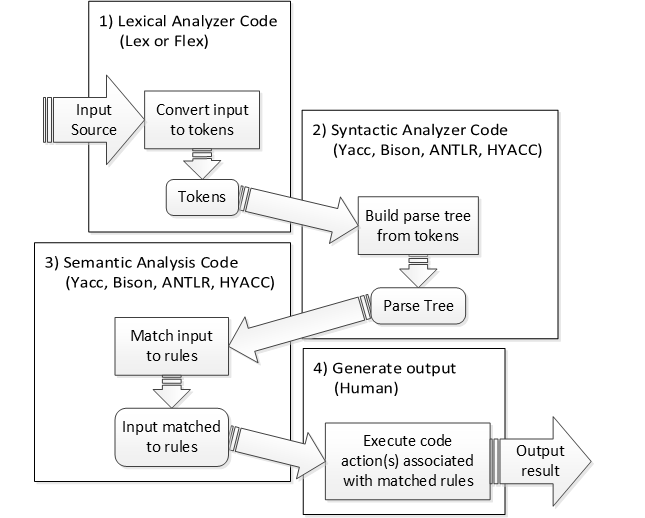
\includegraphics[width=0.9\textwidth]{figures/TraditionalCodeGenProcess.png}
\caption{Traditional code generation process using a lexical analyzer generator in conjunction with a parser generator and actions code.}
\label{fig:TraditionalCodeGenProcess}
\end{figure}

\indent
All of these parser generators provide an effective means to reduce human interaction with code (figure~\ref{fig:TraditionalCodeGenProcess}).  They have the added benefit of generating logical and syntactically correct code as long as the grammar is correct.  On the other hand, the input grammars used by these parser generators cannot be used for lexical analysis of the parser input.  Moreover, code actions that generate output are not provided as part of the input grammar.  These actions must be manually written and inserted into the code generated by the parser generator.
